\section{Exercise 1}

\subsection{}


European option values under a Black-Scholes model with a time-dependent volatility function $\sigma(t)$ are identical to the corresponding option values obtained by a log-transformed model based on the equivalent constant volatility $\sigma_*$. This equivalence arises from matching the first two moments of the log-price distribution

\begin{align*}
\mathbb{E}[\log S(T)] &= \log S_0 + \int_0^T \left(r - \frac{1}{2} \sigma^2(t)\right) dt = \log S_0 + \left(r - \frac{1}{2} \sigma_*^2\right) T \\
\mathrm{Var}[\log S(T)] &= \int_0^T \sigma^2(t) dt = \sigma_*^2 T.
\end{align*}

This ensures identical marginal distributions for the two processes at maturity, although their transitional distributions may differ. The equivalent constant volatility $\sigma_*$ is given by:
\begin{equation}
\sigma_*^2 = \frac{1}{T} \int_0^T \left(0.6 - 0.2 e^{-1.5t}\right)^2 dt = \frac{1}{T}\left(0.36T + \frac{0.24}{1.5}(1 - e^{-1.5T}) - \frac{0.04}{3}(1 - e^{-3T})\right)
\end{equation}
which simplifies to:
\begin{equation}
\sigma_* = \sqrt{0.36 + \frac{0.16}{T}(1 - e^{-1.5T}) - \frac{0.04}{3T}(1 - e^{-3T})}
\label{eq:sigma_star}
\end{equation}

\begin{figure}[h!]
    \centering
    \begin{minipage}{0.42\linewidth}
        \centering
        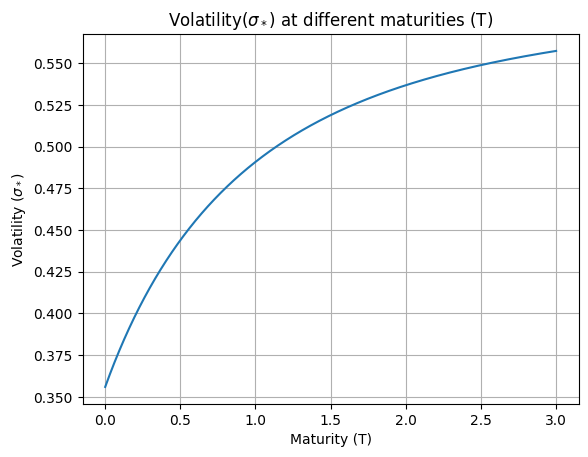
\includegraphics[width=1.05\linewidth]{Exercise_set_02/img/01A_Volatility.png}
        \caption{Value of $\sigma_*$ for different maturities T}
        \label{fig:volatility}
    \end{minipage}%
    \hfill
    \begin{minipage}{0.58\linewidth}
        \centering
        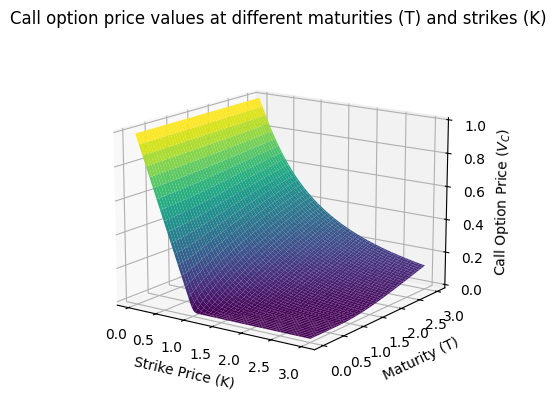
\includegraphics[width=0.8\linewidth]{Exercise_set_02/img/01A_Vc.png}
        \caption{$V_C$ vlue for different maturities T and strikes K}
        \label{fig:vc}
    \end{minipage}
\end{figure}
The European call option price at time $t=0$ under this GBM model with equivalent constant volatility $\sigma_*$ is obtained via the standard Black–Scholes formula using:
\begin{equation}
V_C(S_0,T,K,r,\sigma_*) = S_0 \Phi(d_1) - Ke^{-rT}\Phi(d_2)
\end{equation}
where
\begin{align*}
d_1 = \frac{\ln\frac{S_0}{K} + \left(r + \frac{\sigma_*^2}{2}\right)T}{\sigma_*\sqrt{T}} \qquad \qquad
d_2 = d_1 - \sigma_*\sqrt{T}
\end{align*}
with $\Phi(x)$ representing the cumulative distribution function (CDF) of the standard normal distribution $\mathcal{N}(0,1)$.

In Figure \ref{fig:vc} a plot of the values of the call option for different strikes and maturities.

\subsection{}